\begin{figure*}
\centering
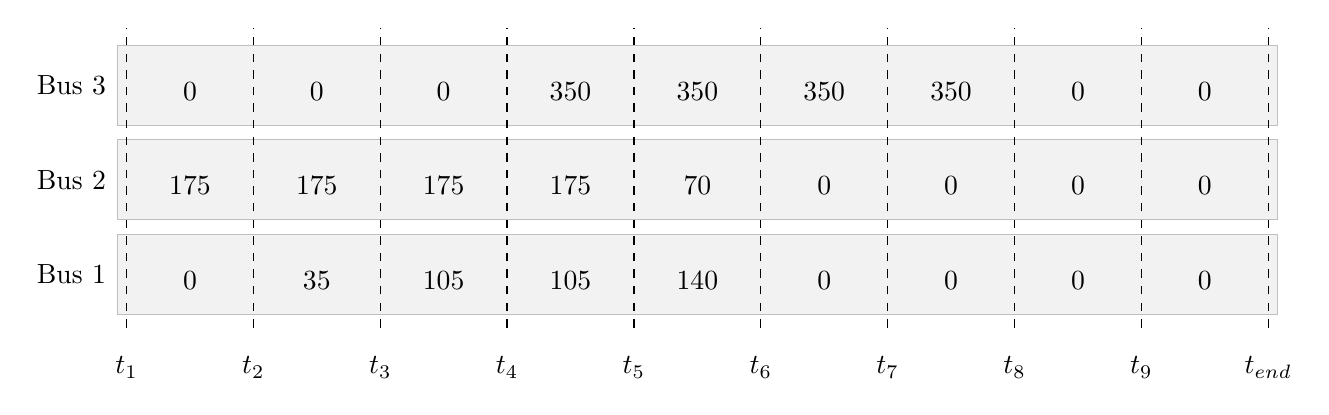
\begin{tikzpicture}
	\node[rectangle, draw=gray!50, fill=gray!10, minimum width=5.8in, minimum height=0.4in](bus1Box) at (7.75,0.8){};
	\node(bus1BoxLabel) at (-0.2, 0.8){Bus 1}; 
	
	\node[rectangle, draw=gray!50, fill=gray!10, minimum width=5.8in, minimum height=0.4in](bus2Box) at (7.75,2){};
	\node(bus1BoxLabel) at (-0.2, 2.0){Bus 2};
	
	\node[rectangle, draw=gray!50, fill=gray!10, minimum width=5.8in, minimum height=0.4in](bus3Box) at (7.75,3.2){};
	\node(bus1BoxLabel) at (-0.2, 3.2){Bus 3};
	
	\foreach \curLab/\preLab[count=\c, evaluate=\c as \pos using {0.5 + (\c - 1)*14.5/9}] in {t_1/t_1, t_2/t_1, t_3/t_2, t_4/t_3, t_5/t_4, t_6/t_7, t_7/t_6, t_8/t_7, t_9/t_8, t_{end}/t_9}
	{
		\node[label=below:$\curLab$](b\c) at (\pos, 0){};
		\node(t) at (\pos, 3.8){};
		\draw[dashed, line width=0.5pt] (b\c.north) -- (t.north); 
		\ifnum\c>1 
			\node(b1Curr) at (\pos, 0.8 - 0.2){};
			\node(b2Curr) at (\pos, 2.0 - 0.2){};
			\node(b3Curr) at (\pos, 3.2 - 0.2){};
			\path(b1Prev.east) -- node(node1\c)[midway, above]{}(b1Curr.west);
			\path(b2Prev.east) -- node(node2\c)[midway, above]{}(b2Curr.west);
			\path(b3Prev.east) -- node(node3\c)[midway, above]{}(b3Curr.west);	
		\fi
			\node(b1Prev) at (\pos, 0.8 - 0.2){};
			\node(b2Prev) at (\pos, 2.0 - 0.2){};
			\node(b3Prev) at (\pos, 3.2 - 0.2){};	
	}
	\path (b9.south) -- node[midway, below=0.1in]{$\hdots$}(b10.south);
	\node at (node12.center){0};
	\node at (node13.center){35};
	\node at (node14.center){105};
	\node at (node15.center){105};
	\node at (node16.center){140};
	\node at (node17.center){0};
	\node at (node18.center){0};
	\node at (node19.center){0};
	\node at (node110.center){0};
	\node at (node22.center){175};
	\node at (node23.center){175};
	\node at (node24.center){175};
	\node at (node25.center){175};
	\node at (node26.center){70};
	\node at (node27.center){0};
	\node at (node28.center){0};
	\node at (node29.center){0};
	\node at (node210.center){0};
	\node at (node32.center){0};
	\node at (node33.center){0};
	\node at (node34.center){0};
	\node at (node35.center){350};
	\node at (node36.center){350};
	\node at (node37.center){350};
	\node at (node38.center){350};
	\node at (node39.center){0};
	\node at (node310.center){0};

\end{tikzpicture}
\caption{An example solution to a 3-bus, 2-charger scenario from the first QP}
\label{fig:solutionExample}
\end{figure*}
